\documentclass[12pt]{article}
\usepackage{amsmath,amsfonts}
\usepackage[cm]{fullpage}
\usepackage{fancyvrb}
\usepackage{graphicx}

\title{January Monthly Problem Set}
\author{Due: 15 January 2018}
\date{}

\begin{document} \maketitle

\begin{enumerate}

\item \textit{JMMO 2017 Question 1}
%  Let $p$ be a prime number such that $3p+10$ is equal to the sum of the squares of six consecutive positive integers. Prove that $36 \mid p-7$.

Let the smallest of the six consecutive integers be $n$. Then we have that
\begin{align*}
    3p + 10 & = n^2 + (n + 1)^2 + (n + 2)^2 + (n + 3)^2 + (n + 4)^2 + (n + 5)^2
    \\
    & = n^2 + (n^2 + 2n + 1) + (n^2 + 4n + 4) + (n^2 + 6n + 9) + (n^2 + 8n + 16)
    + (n^2 + 10n + 25) \\
    & = 6n^2 + 30n + 55,
\end{align*}
and so we have that $p = 2n^2 + 10n + 15$. We thus wish to show that $p - 7 =
2n^2 + 10n + 8$ is divisible by $36$. Note that
\[
    2n^2 + 10n + 8 = 2(n + 1)(n + 4).
\]
Since exactly one of $(n + 1)$ and $(n + 4)$ is even, we have that $p - 7$ is
divisible by $4$. To show that it is also divisible by $9$, it is enough to show
that each of $(n + 1)$ and $(n + 4)$ is divisible by $3$, or, equivalently, that
$n$ is congruent to $2$ modulo $3$. 
        
Suppose that $n$ is not congruent to $2$ modulo $3$. If $n$ is divisible by $3$,
then clearly so is $p = 2n^2 + 10n + 15$, and hence we must have that $p = 3$.
But then $3p + 10 = 19$ is not a sum of six consecutive squares, a
contradiction. If, instead, $n \equiv 1 \pmod 3$, then we have that
\[
    p = 2n^2 + 10n + 15 \equiv 2 \cdot 1 + 10 \cdot 1 + 15 \equiv 0 \pmod 3
\]
and so we again must have that $p = 3$, which is again a contradiction. Thus $n
\equiv 2 \pmod 3$, as required.
        

 
\item % Swiss 2017 Q1
% Let $A$ and $B$ be points on a circle $k$ with centre $O$ such that $AB > AO$. Let $C \neq A$ be the second intersection point of the angle bisector of $\angle OAB$ with $k$. Let $D \neq B$ be the intersection of the line $AB$ with the circumcircle of $OBC$. Prove that $AD = AO$.
Since $OC = OA$ (radii), we have that $\angle ACO = \angle OAC = \angle CAB$.
Since $OA = OB$, we then have that $2\angle ACO = \angle OAB = \angle ABO$, and
since $DBCO$ is a cyclic quadrilateral, this is equal to $\angle DCO$. It
follows that $\angle DCA = \angle ACO$, and so in triangles $\triangle OAC$ and
$\triangle DAC$, we have that $\angle OAC = \angle CAD$, $\angle DCA = \angle
ACO$, and $AC$ is common, and so $\triangle OAC \cong \triangle DAC$, giving us
that $AD = AO$.

\begin{center}
    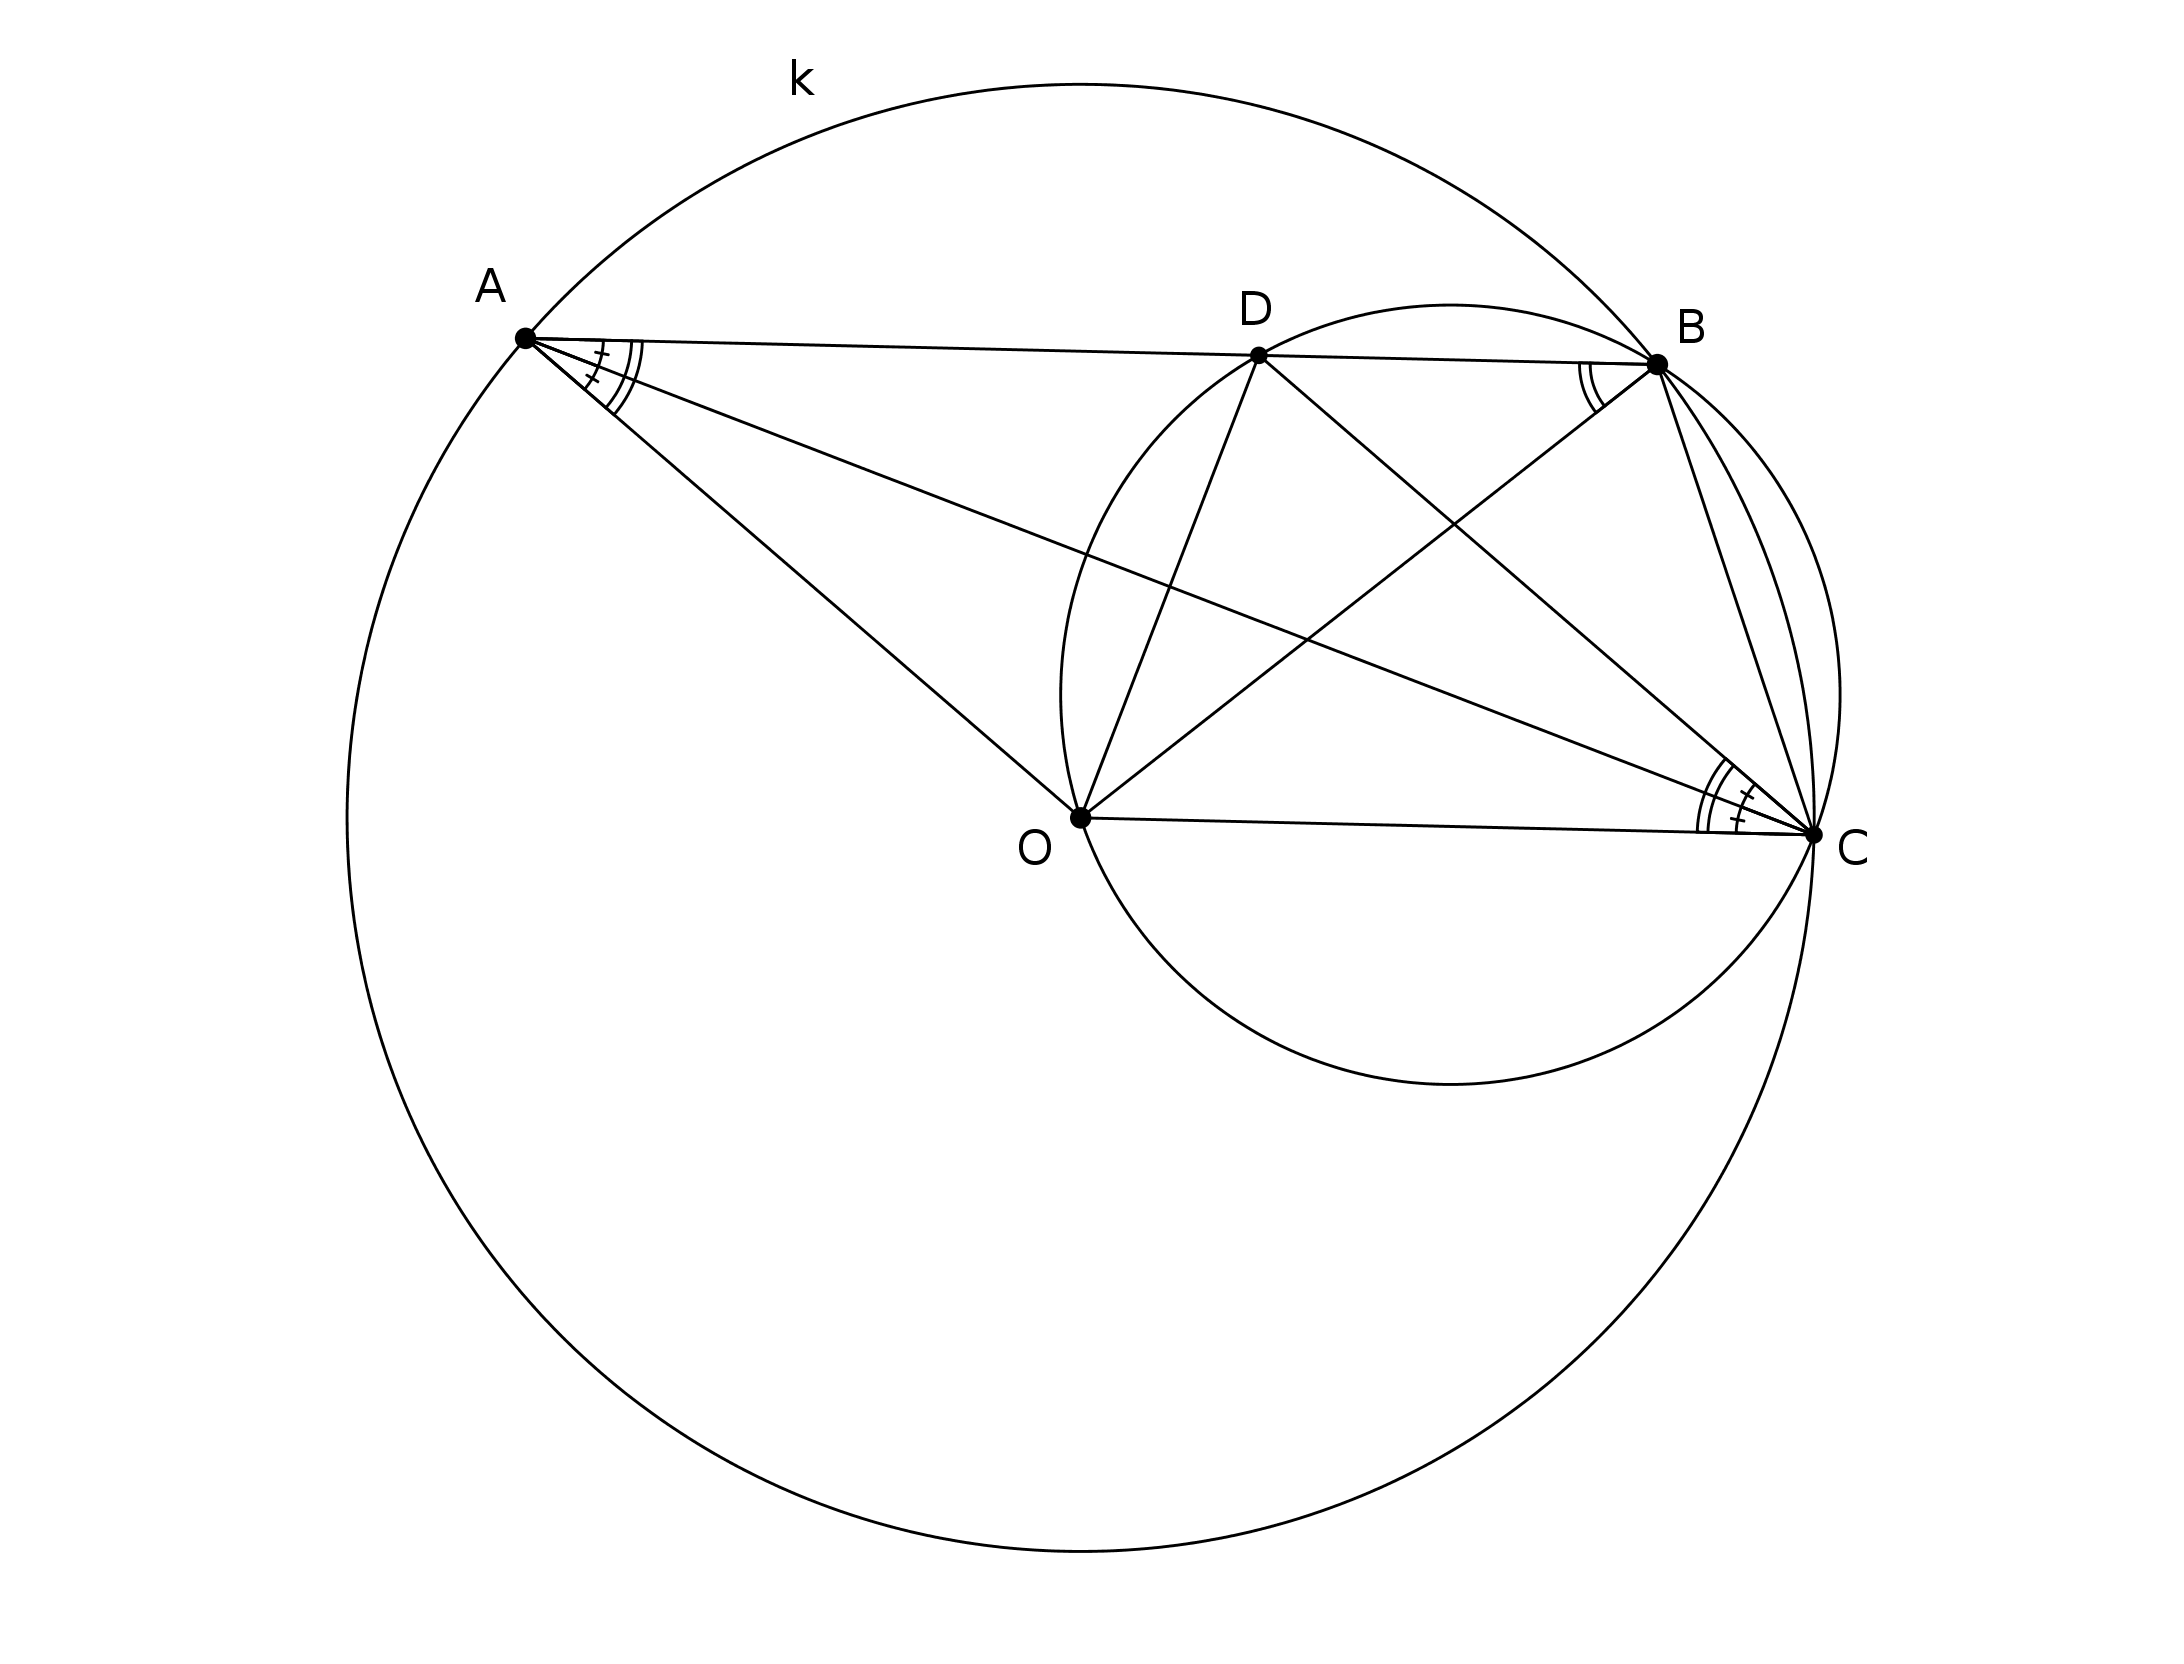
\includegraphics[width=0.5\textwidth]{january_q2.png}
\end{center}

\item % Croatia
% Find all functions $f : \mathbb{R} \to \mathbb{R}$ such that
%  \[ xf(x) - yf(y) = (x - y)(f(x + y) - xy) \]
% for all real numbers $x$ and $y$.
Let $g : \mathbb{R} \longrightarrow \mathbb{R}$ be the function defined by
\[
    g(x) = f(x) - x^2 - a x - b,
\]
where $a = f(1) - f(0) - 1$, and $b = f(0)$. Note that this gives us that $g(0)
= g(1) = 0$.

The functional equation then becomes
\begin{align*}
    xg(x) & + x^3 + ax^2 + bx - yg(y) - y^3 - ay^2 - by \\
    & = (x - y)(g(x + y) + (x + y)^2 + ax + ay + b - xy) \\
    & = (x - y) g(x + y) + a(x^2 - y^2) + b(x - y) + (x - y)(x^2 + xy + y^2) \\
    & = (x - y) g(x + y) + a(x^2 - y^2) + b(x - y) + x^3 - y^3,
\end{align*}
which is equivalent to
\begin{equation} \label{eqn:functional3}
    xg(x) - yg(y) = (x - y) g(x + y)
\end{equation}
for all real numbers $x$ and $y$.

Letting $y = -x$, we get that
\[
    xg(x) + xg(-x) = 2x g(0) = 0
\]
and so for $x \neq 0$, we have that $g(-x) = -g(x)$. Since $g(0) = 0$, this also
holds for $x = 0$. This gives us that
\[
    xg(x) - yg(y) = xg(x) + yg(-y)
\]
for all real numbers $x$ and $y$.

Replacing $y$ with $-y$, in equation \ref{eqn:functional3}, we find that
\[
    xg(x) + yg(-y) = (x + y) g(x - y).
\]
We see that
\[
    (x + y) g(x - y) = (x - y) g(x + y)
\]
for all real numbers $x$ and $y$. Letting $x = y + 1$, we see that
\[
    0 = (2y + 1) g(1) = g(2y + 1)
\]
for all real numbers $y$, and so we see that $g$ must be identically $0$. It
follows that
\[
    f(x) = x^2 + ax + b
\]
for all real numbers $x$.

All functions of this form do indeed satisfy the functional equation, since if
$f(x) = x^2 + ax + b$, then we have that
\begin{align*}
    xf(x) - yf(y) & = x^3 + ax^2 + bx - y^3 - ay^2 - by \\
    & = (x^3 - y^3) + a(x^2 - y^2) + b(x - y) \\
    & = (x - y)(x^2 + xy + y^2 + a(x + y) + b) \\
    & = (x - y)((x + y)^2 - xy + a(x + y) + b) \\
    & = (x - y)(f(x + y) - xy)
\end{align*}
as required.


\item % P Soberon, Problem-Solving Methods in Combinatorics (ladybird --> cat)
% On a 2017x2017 board, some of the squares are occupied by a single cat; the rest of the squares are empty. The cats move, never leaving the board, according to the following rules: every second, each cat moves to a neighbouring square, either horizontally (to the square to its immediate left or right) or vertically (to the square below or above its current square); a cat which makes a horizontal move must move vertically on its next move, and a cat which makes a vertical move must move horizontally on its next move. Determine the smallest number of cats such that regardless of their initial positions and their chosen paths, we may ensure that two of them will eventually find themselves in the same square, at the same moment.


\item % German NMO 2016 Second Round Q4
% Each side of a regular dodecahedron detmines a plane in a unique way. These planes divide the space into a finite number of distinct parts. Determine the number of these parts.
%
%\small{Remark: These planes or parts of them are not considered as parts of the space.}


\item % Dutch TST 2016
%Find all functions $f: \mathbb{R} \to \mathbb{R}$ satisfying
%  \[ f(xy-1) + f(x)f(y) = 2xy-1 \]
%for all $x,y\in R$.

\item % Hard Dutch IMO Selection 2016
%Let $\Gamma_1$ be a circle with centre $A$ and $\Gamma_2$ be a circle with centre $B$ such that $A$ lies on $\Gamma_2$. On $\Gamma_2$ there is a (variable) point $P$ not lying on $AB$. A line through $P$ is a tangent of $\Gamma_1$ at $S$, and it interesects $\Gamma_2$ again in $Q$, with $Q$ and $P$ lying on the same side of $AB$. A different line through $Q$ is tangent to $\Gamma_1$ at $T$. Moreover, let $M$ be the foot of the perpendicular to $AB$ through $P$. Let $N$ be the intersection of $AQ$ and $MT$.
%
%Prove that $N$ lies on a line independent of the position of $P$ on $\Gamma_2$.

\item % Med-Hard? Dutch IMO Selection 2016
%Let $k$ be a positive integer, and let $s(n)$ denote the sum of the digits of $n$. Show that among all positive integers with $k$ digits, there are as many numbers $n$ satisfying $s(n) < s(2n)$ as there are numbers $n$ satisfying $s(n) > s(2n)$.

\end{enumerate}

\vfill

\centering
\begin{BVerbatim}
\end{BVerbatim}

\end{document}
